\subsection{磁気赤道域における潮汐効果の関係}
\label{sec:tidal_effects}
月潮汐（Lunar tide）は、磁場変動の影響を与える要因の一つとして知られている。
\citeauthor{Fujimoto2019} \citeyear{Fujimoto2019}は、地磁気赤道域（ANC）におけるEUELの半日周期変動成分（semidiurnal variation）を解析し、月齢（Lunar age）との関係を調査した。

その結果、Lunar age = 6～9 および 18～21 の期間において、昼間側のEUELが平均値よりも小さくなる傾向が確認された（図\ref{fig:anc_euel_lunar_age}）。
これら期間において潮汐効果に起因する西向き電流が卓越し、背景の東向き電流を打ち消す方向に働くため、観測される磁場変動が抑制されると考えられる。

\begin{figure}[htbp]
  \centering
  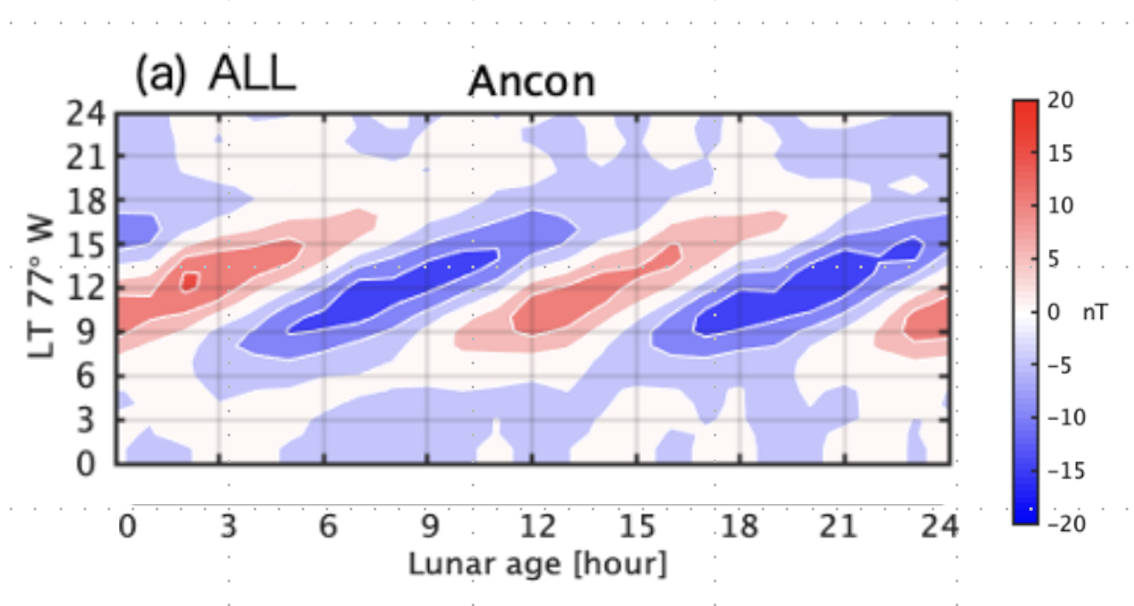
\includegraphics[width=0.8\linewidth]{figures/anc_euel_lunar_age.png}
  \caption{Dip領域(ANC)におけるEUELの半日周期変動成分の平均値からの偏差（\citeauthor{Fujimoto2019} \citeyear{Fujimoto2019}）。赤色は平均より大きく、青色は平均より小さいことを示す。}
  \label{fig:anc_euel_lunar_age}
\end{figure}
